\chapter{Learning user preferences in object placement}
\label{chapter: object}

As robots achieve long term autonomy and they intend to stay longer in human environments, they should be able to adapt quickly to the corresponding environments and the user.  In a series of interviews to understand the needs of people with robots \cite{pantofaru_exploring_2012} concludes, one of the
expectation from robots was help in organizing things based on the user preferences. Since they are service robots its acceptable for a new robot to ask for help from its user in the initial days it moves to a new home, for eg. Where to find a cup?. But as the robot stays longer in a home it becomes less acceptable that the robots ask the user for the same questions, i.e. they should have the capabilities to learn from previous information provided by the user. Robots should also be able to reason and learn from its own observations of the user and the environment. It should be have mechanisms to generate new knowledge about the user and environment from all information gathered. For example, the robot can learn about the user preferences in the cutlery used to setup a breakfast table from previous days observations of breakfast tables. In this chapter we look at such one example of knowledge generation based on previous observations, for learning the user preferences in object placement.

The main advantage of learning user preference about object placement would be in object search. In classical object search, the search is improved based on the knowledge of object locations in a generic home (For eg: cups are found in kitchen, books in shelves)\cite{samadi_using_2012, joho_learning_2011}. Another use of the user preference will be in organizing the home. Here the robot should know what are the objects default locations, so that the robot can place any misplaced objects back to their locations. Understanding user preferences in organizing objects in home has 
been studied by  \cite{abdo_collaborative_2014}, where robots learn about user
preferences in organizing objects, based on the data collected is via crowd-sourcing.  From practical experience we know that even though homes have same base structure in space but the usage of the space is based on the user preferences. Each home is different from other home because of the humans which reside in them use it according to their likes (For eg: some users the keep books on the study table and not on shelves). The proposed methods in this chapter will try to make the robot learn these user preferences specific to each home. So rather than the robot learning object locations in a generic home the proposed methods shall learn object locations in a specific home.


\begin{figure}[htp]
\centering
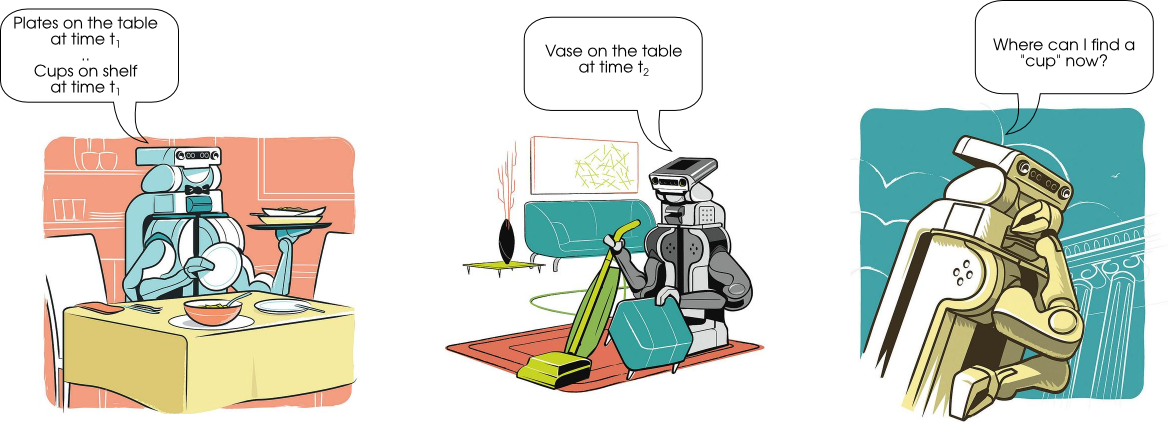
\includegraphics[scale=0.4]{pictures/scenario.png}
\caption[Example scenario of robot recording objects location and time]{Robot recording objects location and time. Based on the
recordings robot making prediction on the location of the cup for current time
Images courtesy : \url{https://www.flickr.com/photos/willowgarage} }
\label{scenario}
\end{figure}

As robots achieve long-term autonomy in dynamic human environments, the robots can collect a lot of observations of it environment and the user. These self collected information can be used by the robot to generate knowledge about the user preferences. We explain this with the help of an illustrative example: 
Consider a domestic robot which has been placed in a home environment with a known map and semantic information of the different locations in the home. The domestic robot while doing its daily activities  makes a record of the objects seen in the environment with their location and time. Now the robot has been asked to bring the coffee mug of the user.
The robot has to make a decision which part of the home it has to go to look for
the coffee mug. The robot can make this decision based on the previous observations of the  location of the coffee mug.
The robot using these previous observations and the time of those observations 
makes a prediction about where the coffee mug can be found at the current time.
Based on previous observation it can be inferred that the coffee mug is usually found in any of the following three location dishwasher/platform/cupboard. Assuming that the time now is morning, from previous observations it can be found that the coffee mug was always found  in the dishwasher. The above example illustrate the main aspects of object location prediction we wish to capture in this chapter.


The model needs to capture two main elements; first that objects in a human environment are not placed randomly but usually have a certain set of places where they are placed. These places of object placement differ from home to home. These object locations entirely depends on the users preferences.  
Second, that human behaviour is related to time i.e. Humans have daily routines  and the object locations are influenced by these routines.
Thus human behaviour not only  has a spatial behaviour but also has a temporal behaviour.
The model will reason on both user preference of the object placement and the
object-time relation.

We now explain a generative Bayesian model which can capture knowledge about user preference in object placement in the environment.

\section{Hierarchical Beta Bernoulli model}

Hierarchical Beta Bernoulli model is a three-level Bayesian model. The basic idea is that observations of the presence of an object at a location(first level), is characterized by a distribution for each hour(second level), which share information via a common latent distribution(third level).

The data are the boolean observation of the object at a location $x_{ij}$ for $i = 1 \dots T$ time periods and then $j = 1, \dots , N$  are the observations.  We assume that the latent pattern that the user will place the object at a  location in a particular period can be represented as a Bernoulli distribution. The number of periods $T$ for our model is fixed to 24 corresponding to the number of hours in a day. 

The conjugate prior for the Bernoulli distribution is the Beta distribution. The model estimates the posterior distribution of $\theta_i$ given our current data and prior beliefs. Our prior beliefs are encoded in the model through the prior $\alpha$ and $\beta$, which represents pseudocounts of what we believe the data should look like – currently taken as same values representing no prior information. The probabilistic graphical model is shown in Figure \ref{bbm}

\noindent
\begin{figure}[htp]

\begin{minipage}{0.3\textwidth}
\centering

\tikz {
 % Define nodes
  \node[latent]                                 (theta) {$\theta$};
  \node[latent, above=of theta, xshift=-1.2cm]  (alpha) {$\alpha$};
  \node[latent, above=of theta, xshift=1.2cm]   (beta) {$\beta$};
  \node[obs, below=of theta]                    (y)     {$x$}; 
  % Connect the nodes
  \edge {alpha,beta} {theta} ; %
  \edge {theta} {y};
  % plates
  \plate {location} {(y)} {location};
  \plate {time} {(theta)(y)(location)} {time};
}

\end{minipage}%
\begin{minipage}{0.7\textwidth}

\begin{equation*}
	\alpha \sim Beta(2,2) ; \beta \sim Beta(2, 2);
\end{equation*}
\begin{equation*}
	\theta \sim Beta(\alpha, \beta);
\end{equation*}
\begin{equation*}
	x = Bernoulli(\theta)
\end{equation*}
\end{minipage}
\caption[Hierarchical Beta Bernoulli graphical model]{Graphical model representation of Hierarchical Beta Bernoulli model. The boxes are ``plates" representing replicates. The outer plates represents hours of a day, while the inner plate represents if object was observed at the location each hour.}
\label{bbm}
\end{figure}

The models are implemented using the PyMC3 probabilistic programming language.

\FloatBarrier
\section{Experiments}

We tested our approach on artificially generated datasets as well as on dataset of object locations collected by a long term robot.
The goal of the experiments were to verify that
\begin{itemize}
    \item the robot is able to learn the object occurrence probability.
	\item the minimum number of observations required to learn a pattern.
	\item the resulting model allows for accurate prediction and control.
\end{itemize}

\subsection{Evaluation of number of observations required}

To quantitatively evaluate the accuracy of the learned model we generated a synthetic dataset of object locations,with know ground truth. The dataset consist of observations made by a mobile domestic robot, of a cup on the counter during different times of the day. The robot while doing its daily chores scans the counter-top of the kitchen. While doing so it records all the instance whenever it finds the cup on the counter. Figure \ref{simulation} shows the ground truth probabilities as well as the count of the different observations generated from the ground truth.

\begin{figure}[htp]
\centering
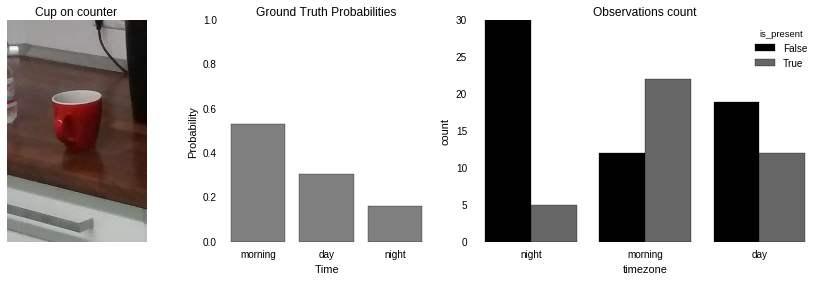
\includegraphics[width=\textwidth]{images/object_simulation.png}
\caption[Simulated object location dataset]{Simulated Object location dataset: Ground truth probabilities of finding a cup on the counter during different times of the day. Observation count of the dataset generated from the ground truth probabilities}
\label{simulation}
\end{figure}

We evaluated the number of observations required to learn a pattern by comparing the learned models  probabilities with the ground truth per time period. The model is trained with increasing number of observations, and the learned probabilities are compared with the ground truth. The procedure is repeated 100 times over different ground truth probabilities. The distance between the two probabilities is shown in Figure \ref{fig:object_simulation_distance}. The dataset is then evaluated for its accuracy by cross validation. Figure \ref {fig:object_simulation_accuracy} plots the accuracy of the model using increasing number of training set. We can observe from the results that with \textbf{25} observations the mean distance is reduced below 0.01 and the accuracy is above 80\%. Thus we can empirically conclude that a minimum of \textbf{25} observations has to be made by the robot to make valid predictions of the object locations. 

\begin{figure}
    \centering
    \begin{subfigure}[b]{0.4\textwidth}
        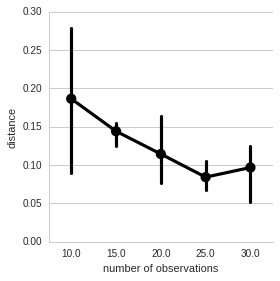
\includegraphics[width=\textwidth]{images/object_simulation_error.png}
        \caption{}
        \label{fig:object_simulation_distance}
    \end{subfigure}
    ~ %add desired spacing between images, e. g. ~, \quad, \qquad, \hfill etc. 
      %(or a blank line to force the subfigure onto a new line)
      \qquad
    \begin{subfigure}[b]{0.4\textwidth}
        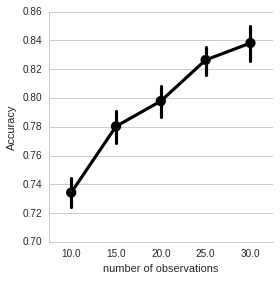
\includegraphics[width=\textwidth]{images/object_simulation_accuracy.png}
        \caption{}
        \label{fig:object_simulation_accuracy}
    \end{subfigure}
    \caption[Evaluation of number of observation required]{Evaluation of number of observation required: Distance between ground truth and learned probabilities \ref{fig:object_simulation_distance}. The accuracy of the learned models using different number of observations \ref{fig:object_simulation_accuracy} }\label{fig:object_simulation_accuracy}
\end{figure}

\FloatBarrier
\subsection{Evaluation of Model Accuracy}

In this section we evaluate the accuracy of the model by using a real world dataset. The KTH Object dataset was collected in the Computer Vision and Active Perception lab at KTH Stockholm, by a SCITOS-G5 mobile robot over  the  course  of  five  weeks.  During  this  time  the  robot conducted  between  two  and  six  autonomous  patrol  runs per  day  (weekends  were  excluded),  visiting  three  specific waypoints  during  each  run.  Upon  reaching  a  waypoint,  the robot  would  execute  a  pan-tilt  sweep  and  collect  data  from its RGB-D sensor; the RGB-D frames collected during one sweep were then registered spatially to form an observation of  that  particular  waypoint  at  that  time.  The  KTH  dataset contains  approximately  100 observations  per  waypoint,  and at  each  waypoint, the  dynamic  elements  of the  environment  using  the  ‘MetaRoom’  method  described in \cite{ambrucs2014meta}. These  dynamic  elements  correspond  to  movable  objects such  as  jackets,  backpacks,  laptops,  chairs,  bottles,  mugs, etc. These dynamic clusters,  manually labelled  to obtain 37 different objects, out  of  which  14  tend  to  appear  and  disappear  periodically \cite{krajnik_wheres_2015}. 

\begin{figure}
    \centering
    \begin{subfigure}[b]{0.21\textwidth}
        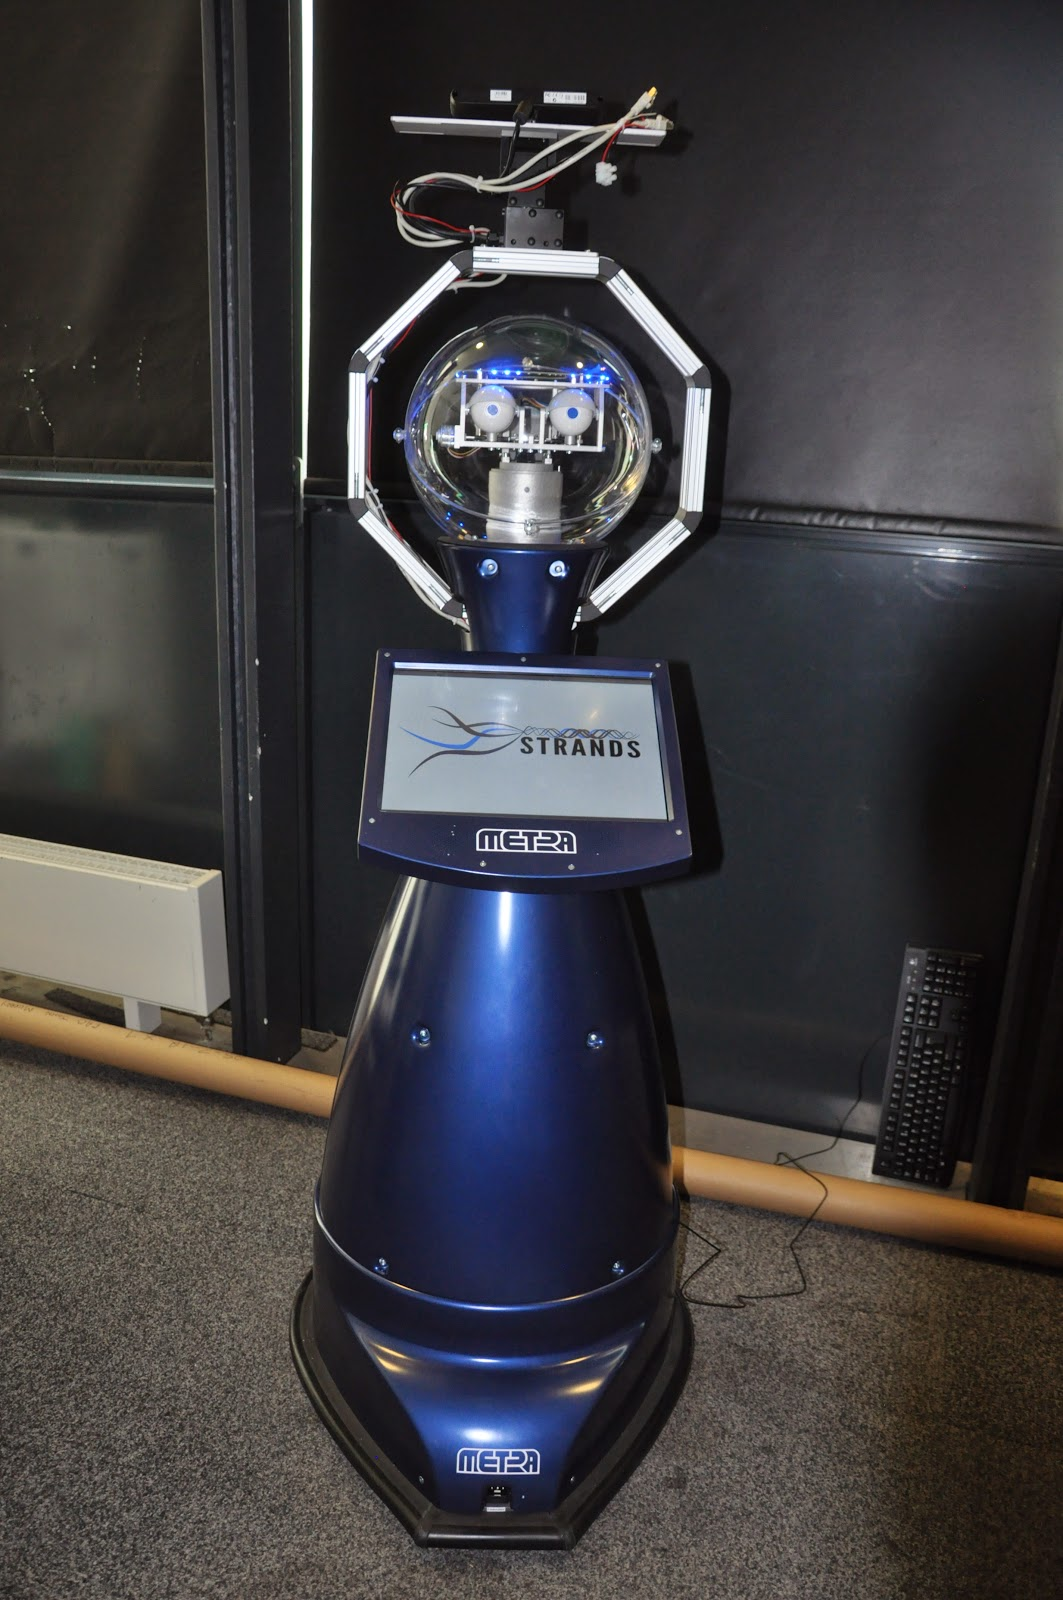
\includegraphics[width=\textwidth]{images/scitos.jpg}
        \caption{}
        \label{fig:scitos}
    \end{subfigure}
    ~ %add desired spacing between images, e. g. ~, \quad, \qquad, \hfill etc. 
      %(or a blank line to force the subfigure onto a new line)
    \begin{subfigure}[b]{0.6\textwidth}
        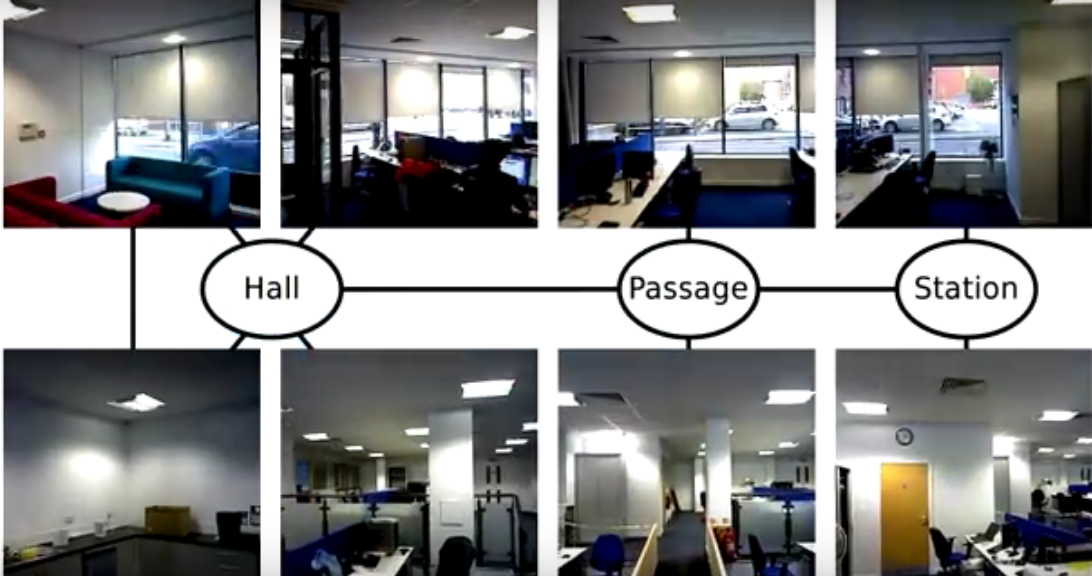
\includegraphics[width=\textwidth]{images/kth-dataset-2.png}
        \caption{}
        \label{fig:robot-view}
    \end{subfigure}
    \caption[KTH dataset collection]{KTH Dataset collection: SCITOS-G5\footnotemark Robot used for data collection \ref{fig:scitos} \protect. Images \footnotemark as seen by the robot at the different waypoints in the lab \ref{fig:robot-view}}\label{fig:kth-dataset}
\end{figure}

\footnotetext{\url{ http://www.hanheide.net/2013/06/brand-new-robot.html}}
\footnotetext{\url{https://www.youtube.com/watch?v=aTr9KD4XMGc }}




The first four weeks of the KTH dataset, is used to train the models and the fifth week is used to evaluate the learned model using cross validation. The accuracy results of 37 objects is plotted in \ref{fig:kth_object_evaluation} . 
Out of the 37 objects \textbf{26} objects have a accuracy rate of above \textbf{70\%} which is denoted by the dotted line. 

\begin{figure}[htp]
\centering
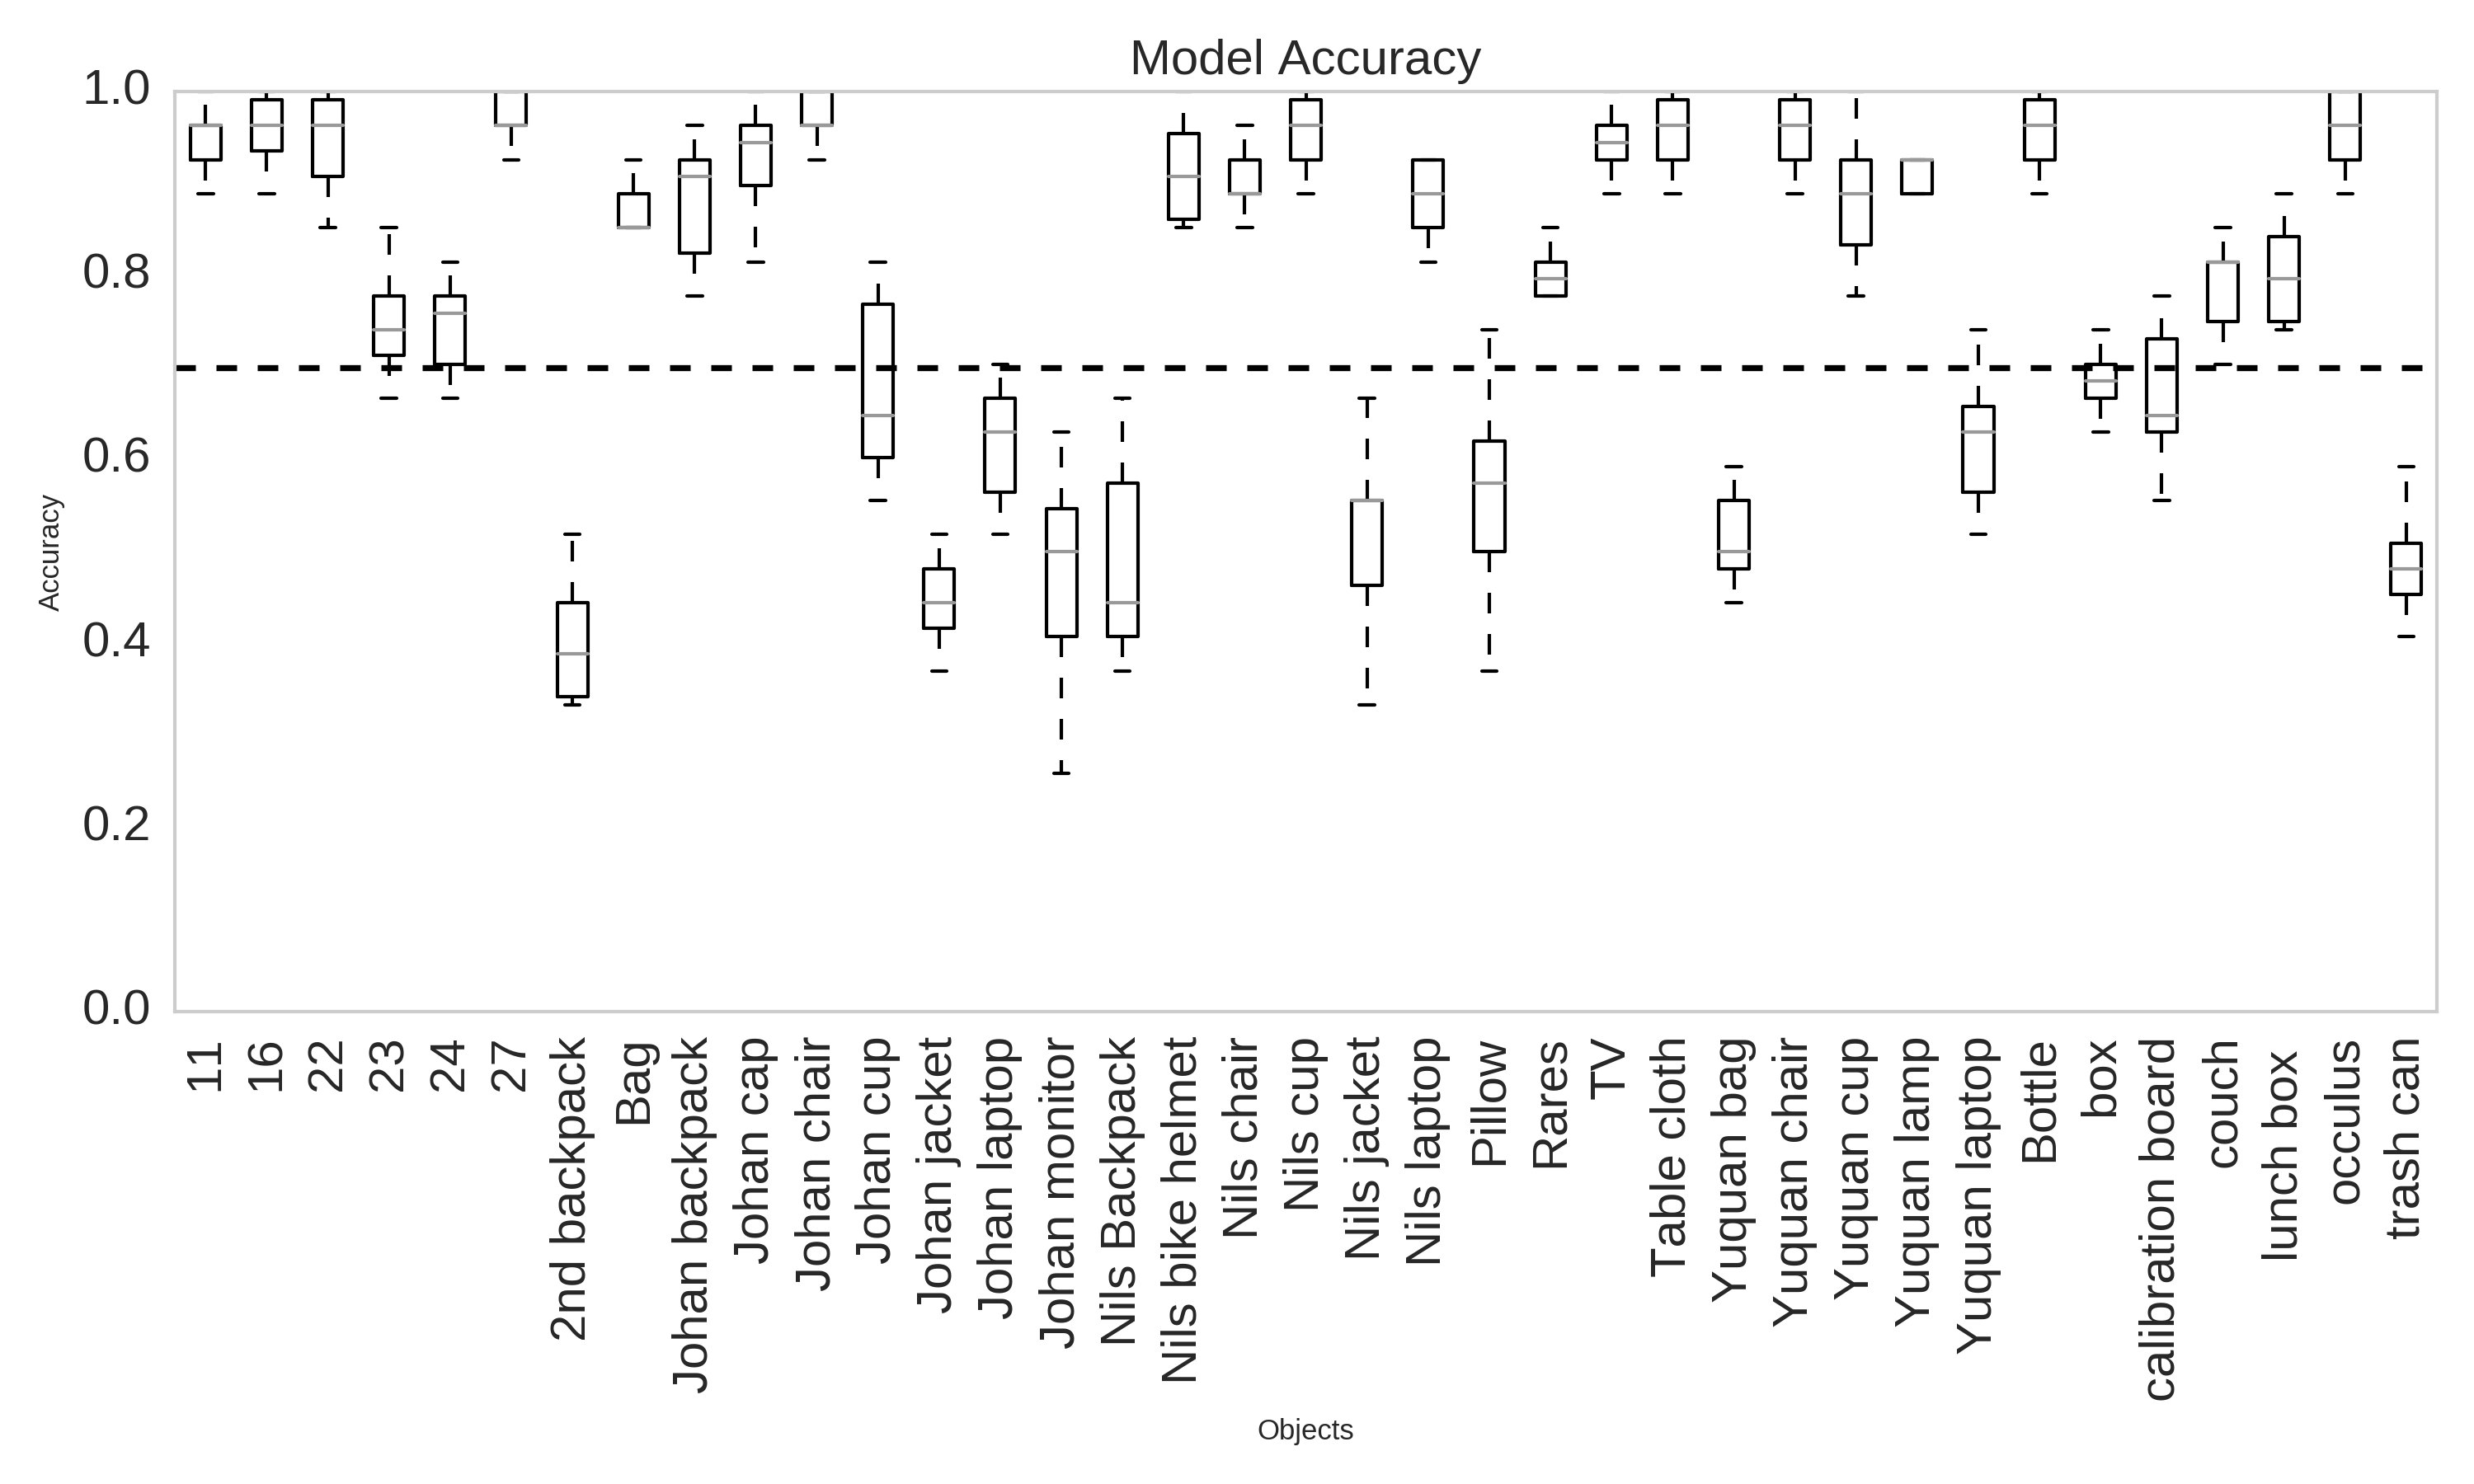
\includegraphics[width=\textwidth]{images/evaluation_kth.png}
\caption[Cross validation results]{Cross validation results. x-axis is the name of the object, y-axis represents the accuracy in predicting the locations of the objects. }
\label{fig:kth_object_evaluation}
\end{figure}

\FloatBarrier
\section{Discussion}
In this chapter, we presented a probabilistic framework for learning the preferences of the user on placing objects in the environment. Our first contribution is to represent the user preferences of object placement using graphical model. Our second contribution is that the graphical model has been implemented using a probabilistic programming language. The robot continuously learns about where the user prefers to keep his objects in the home from the set of object location observations. Since the observations are not continuous trace but just random instances of the objects, the model was designed to be able to capture the latent knowledge in the placement preferences from such sporadic observations.

We have shown by evaluation that the robot needs around 25 observations for gaining knowledge about the object in that location. As seen from evaluation objects which are not moved very often are learned very easily by our models using very less observations. The model performs badly when there is no preference in the user placement i.e. the user places the objects randomly. 
From the real world experiments we can conclude that a majority of the objects in our home environments are rarely moved by the user, therefore our models are able to learn and predict accurately for most of the objects. 
The approaches here capture knowledge about each object in each location separately, we will see in chapter \ref{chapter:Human location} how knowledge about multiple locations of the object can be captured in a single model.
